% !TEX root = ../Rulebook.tex

\newpage
\section{Line Following Test}

\subsection{Purpose and Focus of the Test}
The purpose of the \iaterm{Line Following Test}{LFT} is to address a common task
for industrial robots - following a plain trajectory. For welding, gluing or
painting processes this is implemented by non-mobile manipulators.  This
challenge extends the complexity and focuses on a combined motion by manipulator
and platform. \par The main goal of the challenge is to show a precise operation of the TCP. A
successful completion includes the detection of the trajectory and the movement
of a pen along the line.

\subsection{Scenario Environment}
The arena used for this test contains basically all elements as for the Basic
Navigation Test. Additionally to environmental elements (walls, service areas,
floor markers, etc.), an object with a contour on a flat surface (see Fig.
\ref{awt_examplecontour}) will be added to one of the service areas. The line is
constructed based on a 8x8 mm grid. The referees affix the printout defining the
trajectory on a manipulation zone with a height of 10 cm. All geometrical
definitions given in Fig.~\ref{fig:manipulation_zone} are considered here too.
The trajectory combines just horizontal or vertical line elements and does not
include loops. An exemplary pdf file is available in the RoboCup@Work repository.

Each participating team is free to choose an appropriate pen type and assemble
them to the TCP.

\begin{figure}[h!]
\begin{center}
\subfloat[Examplary TCP equiped with a pen]{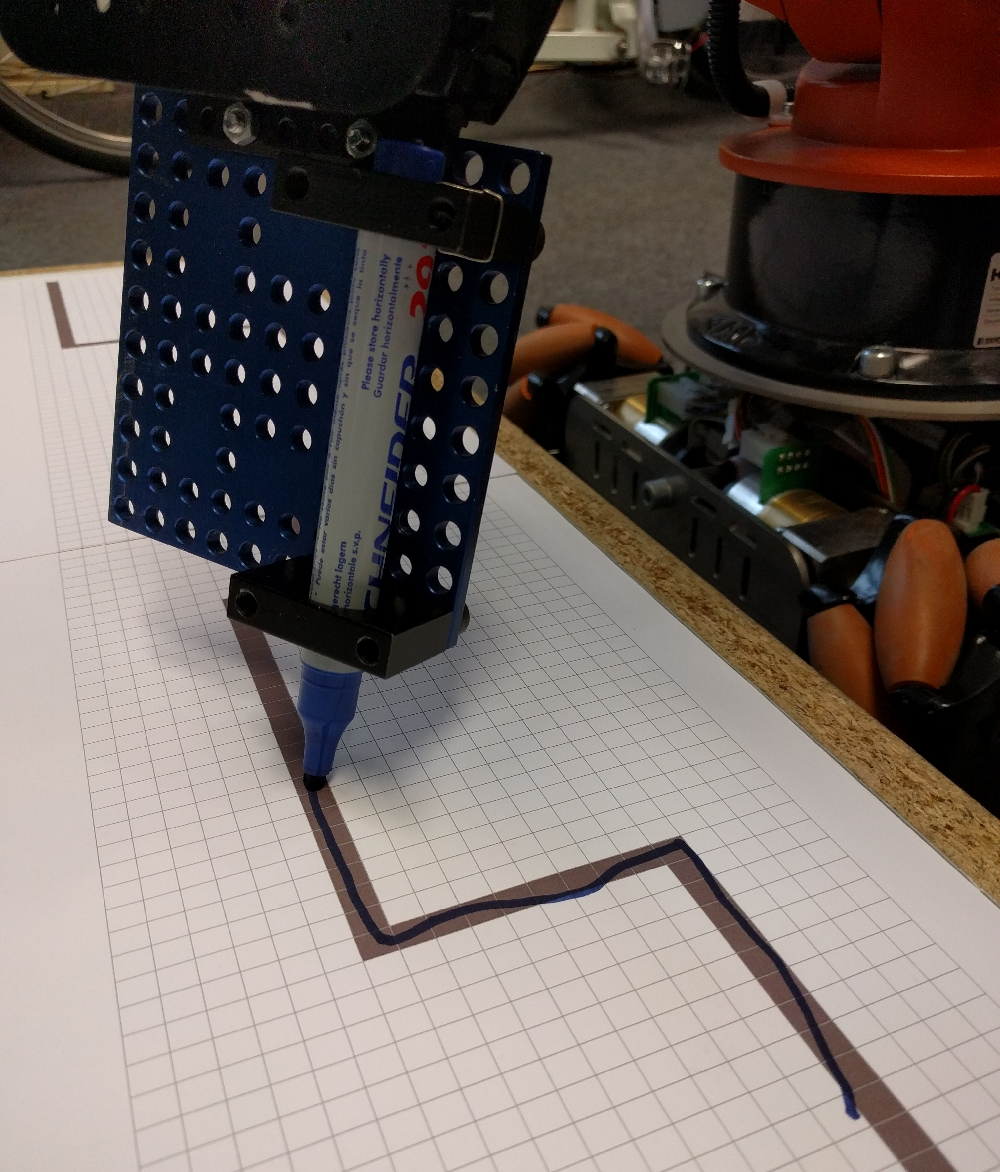
\includegraphics[height = \textwidth/3]{./images/LFT_setup}}
\hspace{0.5cm}
\subfloat[Top view perspective on the test]{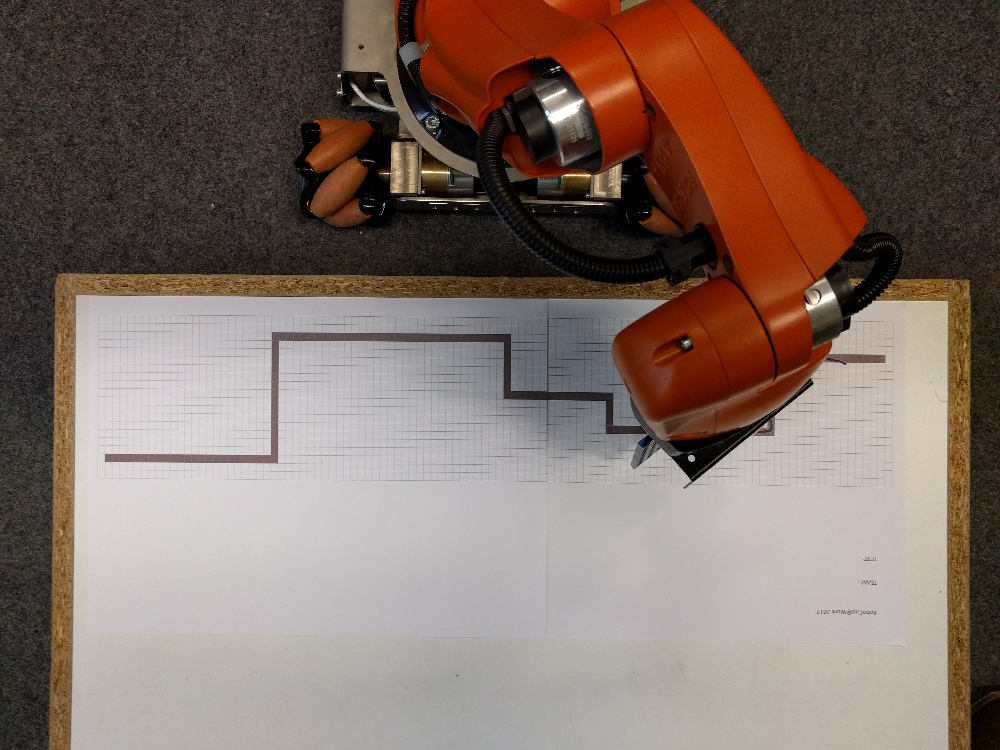
\includegraphics[height = \textwidth/3]{./images/LFT_configuration}}
\end{center}

\caption{Examplary configuration of the trajectory}
\label{awt_examplecontour}
\end{figure}


\subsection{Task}
The task consists of navigating to the specified location and then
moving the pen along the defined contour. 
\par
The task specification consists of the specification of the workstation place (e.g. \texttt{WS09}).

\subsection{Rules}
The following rules have to be obeyed:

\begin{itemize}
\item A single robot is used. 
\item The robot has to start from outside the arena and to end in the final.
\item The order in which the teams have to perform will be determined by a draw.
\item The given trajectory is equal for all teams.
\item At the beginning of a team's period, the team will get the task specification.
\item The run is over when the robot reached the final place or the designated time has expired.
\end{itemize}

\subsection{Scoring}
The referees count the number of grids within the area of the correct line and
grids with pen traces outside. At least 25 coherent grid elements have to be
identified for a valid run!

\begin{itemize}
\item 10 points are awarded for each marked grid within the given trajectory
\item -5 points for every grid element outside of the gray contour
\end{itemize}

\begin{figure}[h!]
\centering
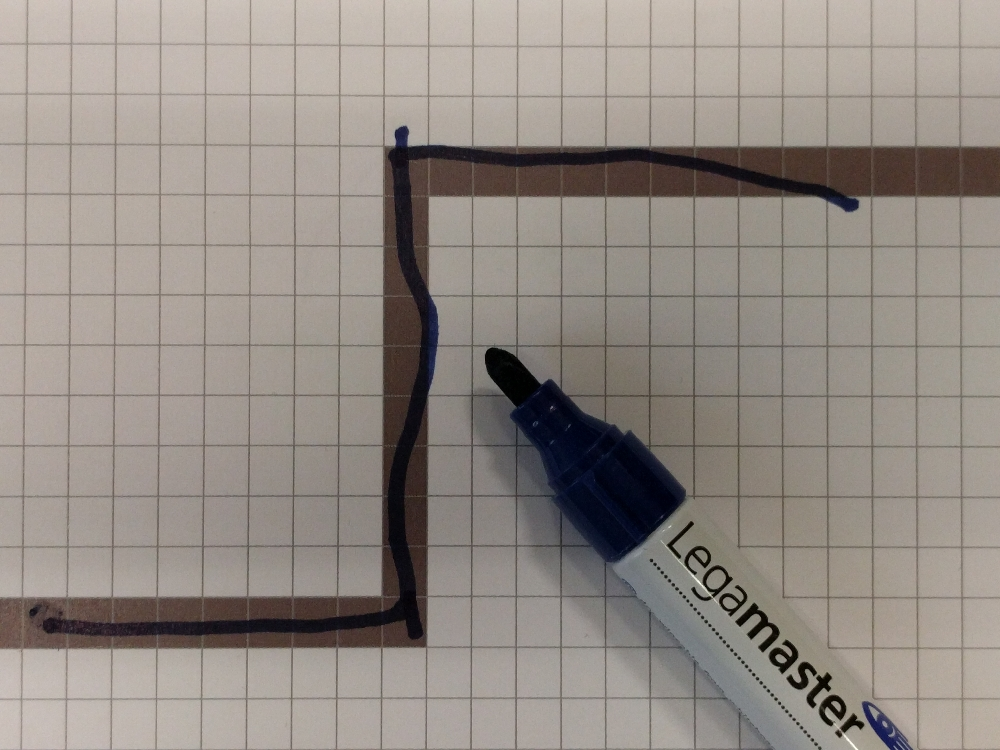
\includegraphics[height = \textwidth/3]{./images/LFT_grid_example}
\caption{Examplary result - 28 valid grid, 4 invalid grids}
\end{figure}
